% !TeX spellcheck = de_DE
\documentclass{uebung_cs}
\usepackage{algo223}
\uebung{3}{}{}
\blattname{Übungen zu Woche 3: Network Flow II}

\usetikzlibrary{arrows.meta}

%%%%%%%%%%%%%%%%%%%%%%%%%%%%%%%%%%%%%%%%%%%%%%%%%%%%%%%%%%%%%%%%%%%%%%%%%%%%
\begin{document}

\begin{exercise}[Residualgraphen zeichnen][\athome]
\
	Betrachte den Fluss~$f$ und das Flussnetzwerk~$(G,s,t,c)$, das in Abbildung~\ref{Fluss} dargestellt ist.
	Zeichne den Residualgraphen $G_f$ und den eingeschränkten Residualgraphen $G_f(3)$.
    \begin{figure}[ht]
		\begin{center}
			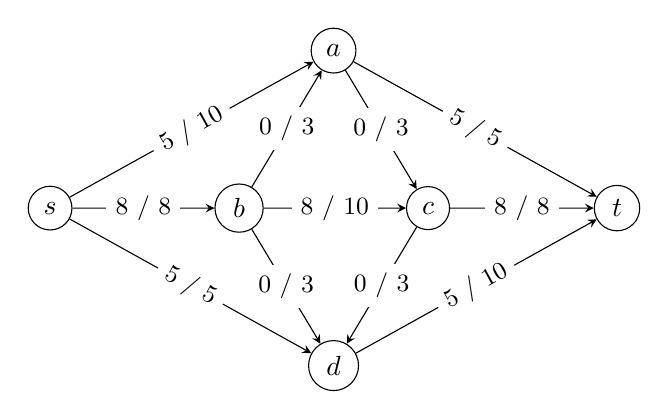
\begin{tikzpicture}[scale=0.8]
				\usetikzlibrary{arrows.meta}
				\node[draw,circle] (v0) at (4.5,  5)	    {$a$};
				\node[draw,circle] (v1) at (0,  2.5)    {$s$};
				\node[draw,circle] (v2) at (3,  2.5)	{$b$};
				\node[draw,circle] (v3) at (6,  2.5)    {$c$};
				\node[draw,circle] (v4) at (9,  2.5)	{$t$};
				\node[draw,circle] (v5) at (4.5,  0)    {$d$};
				
				\def\list {v1/v0/5/10, v1/v2/8/8, v2/v3/8/10, v3/v4/8/8, v0/v4/5/5}  % list elements
				\foreach \u\v\flow\weight in \list
				{	\draw[-stealth] (\u) -- (\v) node [fill=white, sloped, midway] {\small \flow\ $/$ \weight};
				}
				\def\vertical {v2/v0/0/3, v2/v5/0/3, v0/v3/0/3, v3/v5/0/3}  % list elements
				\foreach \u\v\flow\weight in \vertical
				{	\draw[-stealth] (\u) -- (\v) node [fill=white, midway] {\small \flow\ $/$ \weight};
				}
				\def\down {v1/v5/5/5, v5/v4/5/10} %list elements
				\foreach \u\v\flow\weight in \down
				{   \draw[-stealth] (\u) -- (\v) node [fill=white, sloped, midway] {\small \flow\ $/$ \weight};
				}
				
			\end{tikzpicture}
			\caption{\label{Fluss}}
		\end{center}
	\end{figure}
\end{exercise}

\begin{exercise}[Edmonds-Karp Algorithmus und capacity-scaling algorithm][\athome]
    % Algorithms and Data Structures 2 - networks2.pdf
    Benutze sowohl den Edmonds-Karp Algorithmus, als auch den \textit{capacity-scaling algorithm}, um in den folgenden beiden Graphen einen maximalen $s$-$t$-Fluss und einen minimalen $s$-$t$-Schnitt zu berechnen. Schreibe für jeden augmentierenden Pfad die zugehörigen Knoten und den Wert, um die der Pfad augmentiert wird, auf.
    
    \begin{figure}[ht]
    	\begin{minipage}[b]{0.5\textwidth}
    		\centering
    		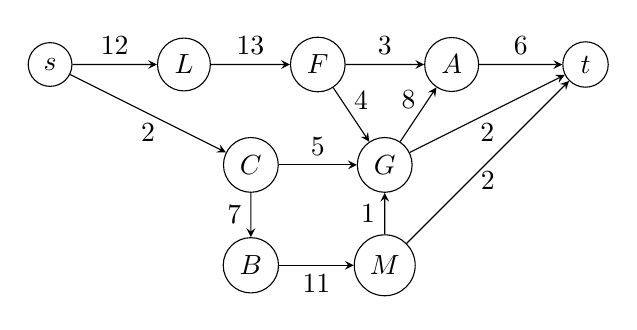
\begin{tikzpicture}[scale=0.85]
			\node[draw,circle] (v0) at (0,  3.5)	{$s$};
			\node[draw,circle] (v1) at (2,  3.5)    {$L$};
			\node[draw,circle] (v2) at (4,  3.5)	{$F$};
			\node[draw,circle] (v3) at (6,  3.5)    {$A$};
			\node[draw,circle] (v4) at (8,  3.5)	{$t$};
			\node[draw,circle] (v5) at (3,    2)    {$C$};
			\node[draw,circle] (v6) at (5,    2)    {$G$};
			\node[draw,circle] (v7) at (3,  0.5)    {$B$};
			\node[draw,circle] (v8) at (5,  0.5)    {$M$};
			
			\def\list {v0/v1/12, v1/v2/13, v2/v3/3, v3/v4/6, v5/v6/5}  % list elements
			\foreach \u\v\weight in \list
			{	\draw[-stealth] (\u) -- (\v) node [midway, above] {\weight};
			}
			
			\def\vertical {v5/v7/7, v8/v6/1 %v0/v4/3, v2/v5/4, v2/v9/4%, v3/v7/7, v6/v10/1, v11/v7/2
            }  % list elements
			\foreach \u\v\weight in \vertical
			{	\draw[-stealth] (\u) -- (\v) node [midway, left] {\weight};
			}
			\def\down {v0/v5/2, v8/v4/2, v6/v4/2, v7/v8/11} %list elements
			\foreach \u\v\weight in \down
			{   \draw[-stealth] (\u) -- (\v) node [midway, below] {\weight};
			}
		
			\draw[-stealth] (v2) -- (v6) node [midway, above, yshift=-1.5, xshift=3.5] {4};
			\draw[-stealth] (v6) -- (v3) node [midway, above, yshift=-1.5, xshift=-3.5] {8};
		\end{tikzpicture}
    	\end{minipage}
    	\begin{minipage}[b]{0.5\textwidth}
    		\centering
    		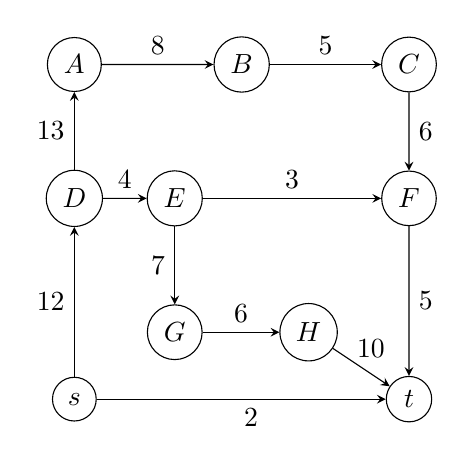
\begin{tikzpicture}[scale=0.85]
			\node[draw,circle] (v0) at (0  ,    0)	  {$s$};
			\node[draw,circle] (v1) at (0  ,    5)    {$A$};
			\node[draw,circle] (v2) at (2.5,    5)	  {$B$};
			\node[draw,circle] (v3) at (5  ,    5)    {$C$};
			\node[draw,circle] (v4) at (0  ,    3)	  {$D$};
			\node[draw,circle] (v5) at (1.5,    3)    {$E$};
			\node[draw,circle] (v6) at (5  ,    3)    {$F$};
			\node[draw,circle] (v7) at (1.5,    1)    {$G$};
			\node[draw,circle] (v8) at (3.5,    1)    {$H$};
			\node[draw,circle] (v9) at (5  ,    0)    {$t$};
			
			\def\list {v0/v4/12, v4/v1/13, v5/v7/7}  % label left from edge
			\foreach \u\v\weight in \list
			{	\draw[-stealth] (\u) -- (\v) node [midway, left] {\weight};
			}
			\def\vertical {v1/v2/8, v2/v3/5, v4/v5/4, v5/v6/3, v7/v8/6}  % label above edge
			\foreach \u\v\weight in \vertical
			{	\draw[-stealth] (\u) -- (\v) node [midway, above] {\weight};
			}
			\def\down {v3/v6/6, v6/v9/5} % label right from edge
			\foreach \u\v\weight in \down
			{   \draw[-stealth] (\u) -- (\v) node [midway, right] {\weight};
			}
			\draw[-stealth] (v8) -- (v9) node [midway, above, yshift=0, xshift=3.5] {10};
			\draw[-stealth] (v0) -- (v9) node [midway, below, yshift=0, xshift=3.5] {2};
		\end{tikzpicture}
    	
    	\end{minipage}
    \end{figure}
\end{exercise}

\newpage
\begin{exercise}[Blutspende][\athome\mittel]
    % KT exercise 7.8
    Statistisch gesehen erhöht sich die Anzahl an Unfällen mit Beginn des Frühlings und damit auch der Bedarf an medizinischen Notfallbehandlungen, sodass auch vermehrt Bluttransfusionen notwendig sind. Stell dir vor, du arbeitest für ein Krankenhaus, das beurteilen muss, ob seine Blutreserven ausreichend sind.

    Beim Blutspenden gibt es eine grundlegende Regel: Eine Person hat in ihrem Blut bestimmte Antigene (du kannst dir Antigene als eine Art molekulare Signatur vorstellen). Bei einer Blutspende kann eine Person nur Blut empfangen, welches die gleichen Antigene hat, wie das eigene. Konkret gesagt unterteilt dieses Prinzip das Blut in vier Gruppen: A, B, AB und 0. Blutgruppe A hat das Antigen A, Blutgruppe B hat das Antigen B, Blutgruppe AB hat beide und Blutgruppe 0 hat keines der Antigene. Demnach können Patienten mit Blutgruppe A nur Blut der Gruppen A und 0, Patienten der Blutgruppe B nur Blut der Gruppen B und 0, Patienten der Blutgruppe 0 nur Blut der Gruppe 0 und Patienten der Blutgruppe AB Blut aller Blutgruppen empfangen.
    \begin{enumerate}
    	\item Das Krankenhaus hat für jede der vier Blutgruppen eine bestimmte Anzahl an ganzen Einheiten vorrätig. Diese Anzahlen sind gegeben durch $s_0,s_A,s_B,s_{AB}\in\N$.
		Außerdem kennt das Krankenhaus den prognostizierten Bedarf $d_0, d_A,d_B,d_{AB}\in\N$ an Blut für die nächste Woche. Entwirf einen effizienten Algorithmus, der entscheidet, ob das vorrätige Blut den prognostizierten Bedarf der nächsten Woche deckt. (\emph{Tipp: \reflectbox{Konstruiere ein geeignetes Flussnetzwerk als Eingabe für Ford-Fulkerson}})
    	\item
		%  Das Krankenhaus prognostiziert für die nächste Woche einen Bedarf von $100$ Einheiten Blut.
		% Die durchschnittliche Verteilung der Blutgruppen über die U.S.-Bevölkerung liegt bei $45\%$ Blutgruppe 0, $42\%$ Blutgruppe A, $10\%$ Blutgruppe B und $3\%$ Blutgruppe AB. Das Krankenhaus möchte wissen, ob seine Vorräte ausreichend sind, wenn $100$ Patienten mit der erwarteten Verteilung über die Blutgruppen behandelt werden müssen. Es sind $105$ Einheiten Blut vorrätig.
		Wir schauen uns nun ein konkretes Beispiel an.
		Die folgende Tabelle gibt den Vorrat und die Nachfrage an Blut an:
    	
    	\vspace{4mm}
    	\begin{center}
    	\begin{tabular}{|c|c|c|}
    	% \hline 
    	Blutgruppe & Vorrat & Nachfrage \\ 
    	% \hline 
    	0 & 50 & 45 \\ 
    	% \hline 
    	A & 36 & 42 \\ 
    	% \hline 
    	B & 11 & 10 \\ 
    	% \hline 
    	AB & 8 & 3 \\ 
    	% \hline 
    	\end{tabular}
    	\end{center}
    	\vspace{4mm}
    	Sind die 105 vorrätigen Einheiten Blut ausreichend, um der Nachfrage von $100$ Einheiten gerecht zu werden? Finde eine Zuordnung, sodass die maximale Anzahl an Patienten behandelt werden kann. Benutze die Idee minimaler Schnitte in einem passenden Flussnetzwerk, um zu begründen, warum nicht alle Patienten behandelt werden können. Stelle außerdem eine allgemeinverständliche Erklärung dieses Umstandes für diejenigen Mitglieder der Krankenhausverwaltung bereit, die ALGO2 nicht belegt haben. (Beispielsweise soll deine Erklärung die Worte \emph{Fluss}, \emph{Schnitt} oder \emph{Graph} nicht in dem Sinne enthalten, wie wir sie in der Vorlesung benutzen.)
    \end{enumerate}
\end{exercise}

\newpage
\begin{exercise}[Weihnachtsbäume]
    % Algorithms and Data Structures 2 - networks2.pdf
    Professor Regloh hat dich beauftragt, die jährliche Weihnachtsfeier für alle Student:innen der Goethe-Universität zu organisieren. Du musst einen Plan erstellen, auf dem die Platzierung der Tische im Casino-Festsaal vermerkt ist. Damit die Brandschutzmaßnahmen eingehalten werden können, hat die Frankfurter Feuerwehr den Festsaal in ein rechteckiges $n \times m$ Gitter aufgeteilt und festgelegt, dass höchstens zwei Tische in jeder Zeile und höchstens ein Tisch in jeder Spalte aufgestellt werden dürfen. Leider liebt Professor Regloh Weihnachtsbäume sehr und hat schon einige aufstellen lassen. Du darfst diese nicht verschieben und kannst einen Tisch nur dort aufstellen, wo noch kein Weihnachtsbaum steht.
    
    \begin{figure}[h]
    \centering
    \begin{minipage}{0.4\textwidth}
    	\begin{tabular}{|c|c|c|c|c|c|c|c|}
    		\hline 
			$\star$ &  &  &  &  &  &  &  \\ 
    		\hline 
	    	& $\star$ & $\star$ &  & $\star$ & $\star$ &  & $\star$ \\ 
	    	\hline 
		    & $\star$ & $\star$ &  & $\star$ & $\star$ &  & $\star$ \\ 
    		\hline 
		    & $\star$ &  & $\star$ &  &  & $\star$ &  \\ 
    		\hline 
    	\end{tabular}
    	\caption{\label{Ohne_Tische}}
    \end{minipage}
    \begin{minipage}{0.4\textwidth}
    	\begin{tabular}{|c|c|c|c|c|c|c|c|}
		    \hline 
    		$\star$ & $T$ &  &  &  &  &  & $T$ \\ 
	    	\hline 
	    	$T$ & $\star$ & $\star$ & $T$ & $\star$ & $\star$ &  & $\star$ \\ 
		    \hline 
    		& $\star$ & $\star$ &  & $\star$ & $\star$ & $T$ & $\star$ \\ 
		    \hline 
    		& $\star$ & $T$ & $\star$ &  & $T$ & $\star$ &  \\ 
	    	\hline 
    	\end{tabular}
    	\caption{\label{Mit Tischen}}
    \end{minipage}
    \end{figure}
     
    \textbf{Beispiel.} Es gilt $n = 4$ und $m = 8$. Die $\star$ stellen Weihnachtsbäume dar und $T$ die Tische. In \cref{Ohne_Tische} ist die Anfangssituation (Weihnachtsbäume positioniert, Tische nicht) dargestellt. In \cref{Mit Tischen} ist eine bestmögliche Positionierung der maximalen Anzahl an Tischen (7) dargestellt.
   
    \begin{enumerate}
    	\item\athome Modelliere das Problem als ein Netzwerkflussproblem. Erkläre, wie du dir das überlegt hast und zeichne den zum oben angegebenen Beispiel passenden Graphen.
    	\item\athome\mittel Gegeben sind $n,m$ und die Platzierung der Weihnachtsbäume. Beschreibe einen Algorithmus, der eine maximale Anzahl an Tischen, die im Festsaal platziert werden können, ausgibt. Analysiere die asymptotische Laufzeit deines Algorithmus und denke daran, die Korrektheit deines Algorithmus zu zeigen.
    	\item\projekt Implementiere deinen Algorithmus in Python, Java, oder C/C\texttt{++}. (In Moodle steht hierfür eine Coderunner-Aufgabe zur Verfügung!)
    \end{enumerate}
\end{exercise}

\begin{exercise}[Fluchtwege][\atschool\mittel]
    % KT exercise 7.14
    Wir definieren das Fluchtproblem wie folgt: Gegeben ist ein gerichteter Graph $G = (V,E)$ (stell dir ein Straßennetzwerk vor). Eine Teilmenge $X \subseteq V$ aller Knoten sind bewohnte Knoten und eine andere Teilmenge $S \subseteq V$ sind sichere Knoten. Du kannst annehmen, dass $X$ und $S$ disjunkt sind. Für den Notfall soll es Fluchtwege von den bewohnten Knoten zu den sicheren Knoten geben. Eine Menge von Fluchtwegen ist als eine Menge von Pfaden in $G$ definiert, sodass
    \begin{enumerate}[i.]
      \item jeder Knoten aus $X$ der Anfang eines Pfades ist,
      \item der letzte Knoten jedes Pfades in $S$ liegt und
      \item die Pfade paarweise keine gemeinsamen Kanten besitzen.   
    \end{enumerate}
    Diese Menge von Pfaden sorgt dafür, dass die bewohnten Knoten sicher evakuiert werden können, ohne dass eine Kante in $G$ überlastet wird.
    \begin{enumerate}
    	\item Zeige, wie bei einer Eingabe von $G, X, S$ in polynomieller Zeit entschieden werden kann, ob eine solche Menge von Fluchtwegen existiert.
    	\item Wir wollen das gleiche Problem wie in Aufgabenteil a)~mit einer strengeren Version von Bedingung iii.~lösen, das heißt die Pfade dürfen keine gemeinsamen Knoten mehr haben.
    	Zeige, wie in polynomieller Zeit entschieden werden kann, ob eine Menge von Fluchtwegen gemäß dieser neuen Bedinungen existiert.
    	
    	Gib außerdem eine Beispiel-Eingabe $G_0, X_0, S_0$ an, für die der Algorithmus aus Aufgabenteil a) \glqq Ja\grqq{} ausgibt und der Algorithmus aus Aufgabenteil b) \glqq Nein\grqq.
    \end{enumerate}
\end{exercise}

\newpage
\begin{exercise}[Eulerkreise in gemischten Graphen][\atschool\note]
    % Algorithms and Data Structures 2 - networks2.pdf
    Ein Eulerkreis ist ein Kreis, der jede Kante genau einmal enthält.
    Es ist bekannt, dass ein stark zusammenhängender Graph einen Eulerkreis genau dann besitzt, wenn jeder Knoten die gleiche Anzahl eingehender und ausgehender Kanten hat.

	\emph{Gemischte Graphen} sind Graphen, in denen einige Kanten gerichtet und einige ungerichtet sind. Wir nehmen an, dass die Graphen schwach zusammenhängend sind, also dass der zugrunde liegende ungerichtete Graph zusammenhängend ist. 
    
    Gib einen Algorithmus an, der entscheidet, ob man allen ungerichteten Kanten eine Richtung zuweisen kann, sodass der dadurch entstehende gerichtete Graph einen Eulerkreis besitzt. Im folgenden Beispiel können die ungerichteten Kanten des gemischten Graphen (\emph{links}) so gerichtet werden (\emph{rechts}), dass ein Eulerkreis entsteht (die Zahlen an den Kanten geben die Besuchsreihenfolge an).

    \begin{figure}[ht]
    	\begin{minipage}[b]{0.5\textwidth}
    		\centering
    		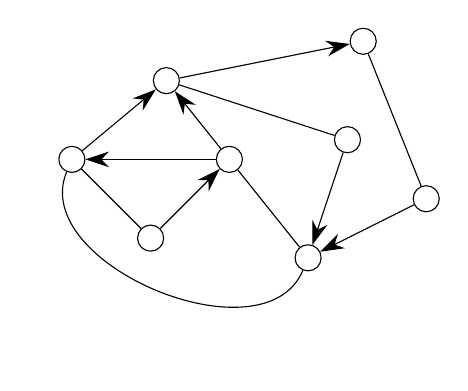
\begin{tikzpicture}
			\node[draw,circle] (v0) at (0,  0)  {};
			\node[draw,circle] (v1) at (1,  -1)  {};
			\node[draw,circle] (v2) at (1.2, 1)  {};
			\node[draw,circle] (v3) at (2,  0)  {};
			\node[draw,circle] (v4) at (3,  -1.25)  {};
			\node[draw,circle] (v5) at (3.5, 0.25)  {};
			\node[draw,circle] (v6) at (3.7,  1.5)  {};
			\node[draw,circle] (v7) at (4.5,  -0.5)  {};
			
			\def\list {v0/v2, v1/v3, v2/v6, v3/v0, v3/v2, v5/v4, v7/v4}  % directed edges
			\foreach \u\v in \list
			{	\draw[-{Stealth[length=3mm, width=2mm]}] (\u) -- (\v);}
			
			\def\vertical {v0/v1, v2/v5, v3/v4, v6/v7}  % undirected edges
			\foreach \u\v in \vertical
			{	\draw[] (\u) -- (\v);}
			
			\path (v0) edge[bend right=90] node [left] {} (v4);
		\end{tikzpicture}
    	\end{minipage}
    	\begin{minipage}[b]{0.5\textwidth}
    		\centering
    		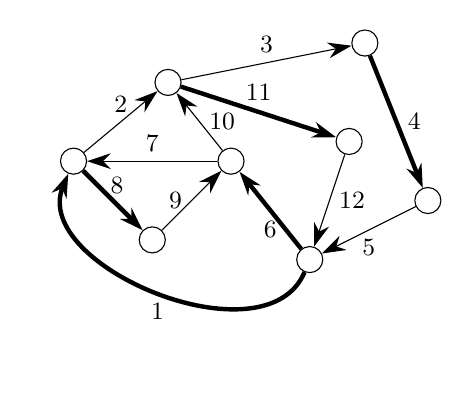
\begin{tikzpicture}
			\node[draw,circle] (v0) at (0,  0)  {};
			\node[draw,circle] (v1) at (1,  -1)  {};
			\node[draw,circle] (v2) at (1.2, 1)  {};
			\node[draw,circle] (v3) at (2,  0)  {};
			\node[draw,circle] (v4) at (3,  -1.25)  {};
			\node[draw,circle] (v5) at (3.5, 0.25)  {};
			\node[draw,circle] (v6) at (3.7,  1.5)  {};
			\node[draw,circle] (v7) at (4.5,  -0.5)  {};
			
			\path (v4) edge[-{Stealth[length=3mm, width=2mm]}, ultra thick, bend left=90] node [font=\small,midway, below] {$1$} (v0);
			\path (v0) edge[-{Stealth[length=3mm, width=2mm]}							] node [font=\small,midway, above] {$2$} (v2);
			\path (v2) edge[-{Stealth[length=3mm, width=2mm]}							] node [font=\small,midway, above] {$3$} (v6);
			\path (v6) edge[-{Stealth[length=3mm, width=2mm]}, ultra thick				] node [font=\small,midway, right] {$4$} (v7);
			\path (v7) edge[-{Stealth[length=3mm, width=2mm]}							] node [font=\small,midway, below] {$5$} (v4);
			\path (v4) edge[-{Stealth[length=3mm, width=2mm]}, ultra thick				] node [font=\small,midway, below] {$6$} (v3);
			\path (v3) edge[-{Stealth[length=3mm, width=2mm]}							] node [font=\small,midway, above] {$7$} (v0);
			\path (v0) edge[-{Stealth[length=3mm, width=2mm]}, ultra thick				] node [font=\small,midway, above,yshift=-1.5, xshift=1.5] {$8$} (v1);
			\path (v1) edge[-{Stealth[length=3mm, width=2mm]}							] node [font=\small,midway, left ] {$9$} (v3);
			\path (v3) edge[-{Stealth[length=3mm, width=2mm]}							] node [font=\small,midway, right] {$10$} (v2);
			\path (v2) edge[-{Stealth[length=3mm, width=2mm]}, ultra thick				] node [font=\small,midway, above] {$11$} (v5);
			\path (v5) edge[-{Stealth[length=3mm, width=2mm]}							] node [font=\small,midway, right] {$12$} (v4);
			
		\end{tikzpicture}
    	
    	\end{minipage}
    \end{figure}
    
    \textit{Hinweis:} Konstruiere einen bipartiten Graphen mit den Knoten aus $G$ auf der einen Seite und den Kanten aus $G$ auf der anderen Seite, und nutze dann den Algorithmus der vorherigen Aufgabe.
\end{exercise}

\begin{exercise}[Puzzle der Woche: Das Zwölf-Münzen Problem][\spass]
	% Algorithms and Data Structures 2 - networks2.pdf
	Vor dir liegen 12 Münzen. 11 davon sind identisch, aber eine Münze ist schwerer oder leichter als der Rest. Du hast eine traditionelle Balkenwaage mit zwei Waagschalen. Um die Waage zu benutzen, legst du eine Münze in jede Schale. Die Waage zeigt dann an, welche der beiden Seiten (und damit welche der beiden Münzen) schwerer ist. Die Balkenwaage darf dreimal benutzt werden, um die andere Münze zu finden und um festzustellen, ob diese leichter oder schwerer ist als der Rest.
\end{exercise}

\end{document}
